\documentclass[addpoints,12pt,answers]{exam}
\usepackage{babel}
\usepackage[top=3cm,bottom=3cm,left=2.5cm,right=2.5cm]{geometry}
\usepackage[utf8]{inputenc}
\usepackage[T1]{fontenc}
\usepackage{booktabs}
\usepackage{graphicx}
\usepackage{csquotes}
\usepackage{paralist}
\usepackage{wasysym}
\usepackage[math]{iwona}
\usepackage{setspace}
\usepackage{enumitem}
\usepackage{multirow}
\usepackage{listings}


\pointpoints{Point}{Points}
\bonuspointpoints{Bonuspunkt}{Bonuspunkte}
\renewcommand{\solutiontitle}{\noindent\textbf{Solution:}\enspace}

\chqword{Frage}
\chpgword{Seite}
\chpword{Punkte}
\chbpword{Bonus Points} 
\chsword{Erreicht}   
\chtword{Gesamt}

\checkboxchar{\Square}
\checkedchar{\CheckedBox}

\pagestyle{headandfoot}
%\runningheadrule
%\firstpageheader{ECO208}{Test 3}{28th Feb, 2022}
%\runningheader{ECO208}{Test 3}{28th Feb, 2022}
%\firstpagefooter{ECO208}{Test 3}{\thepage\,/\,\numpages}
%\runningfooter{ECO208}{Test 3}{\thepage\,/\,\numpages}
\doublespacing

\begin{document}
	\vspace*{3em}
	
	\makebox[\textwidth]{ECO 209  Assignment 3}
	\makebox[\textwidth]{Name:\enspace\hrulefill}
	
	\vspace*{3em}
	
	\begin{enumerate}[label=\textbf{\arabic*.}, itemsep=15pt]
		
		
%		\item  \textbf{(15  pts)}  Use the balance sheet below:
%		
%		\begin{figure}[htbp!]
%			\centering
%			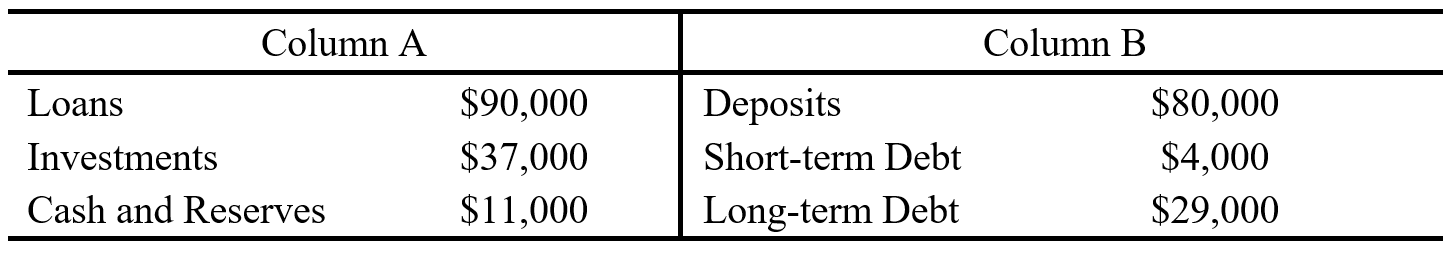
\includegraphics[width=0.8\linewidth]{figure/t-balance_1}
%
%		\end{figure}
%		Currently, the bank must maintain a capital-to-asset ratio of 5\%.
%		
%		\begin{enumerate}[label=(\alph*)]
%			\item \textbf{(2  pts)}  What is the bank’s net worth?
%			\item \textbf{(2  pts)}  What is this bank’s leverage ratio?
%			\item \textbf{(3  pts)}  Does the bank meet the capital requirement? If so, what is the amount of excess capital held by the bank? If not, how much does the bank needs to augment its net worth by injecting more cash?
%			\item \textbf{(3  pts)}  Now, the new financial regulator requires that banks maintain a 20\% capital-to-asset ratio. If no new capital is to be injected, what actions should the bank take?
%			\item \textbf{(5  pts)}  Before the bank can take any action and the bank encounters an investment shock resulting in a \$5,000 decrease in investments, what is the current net worth of the bank? Explain how this situation could potentially pose further challenges if all the banks in the market faced similar investment shock and are obligated to meet the 20\% capital to asset ratio requirement, within a range of 50-100 words.
%		\end{enumerate}
%		\clearpage
%		\textbf{Solution}
%		\begin{enumerate}[label=(\alph*)]
%			\item Net worth = Asset - Liability
%			\[\textit{Net worth} = 90000+37000+11000-(80000+4000+29000) = 25000\]
%			\item $\textit{Leverage Ratio} = \frac{\textit{total liabilities}}{\textit{net worth}} = \frac{113000}{25000} = 4.52$
%			\item The capital to asset ratio is $\frac{25000}{138000} = 0.181$. The bank meet the capital requirement. It has an excess capital of $25000-138000\times 5\% = 18100$
%			\item The bank would have to sell its investment (or use its cash and reserves) to repay its debt. 
%			
%			\[\frac{138000-113000 }{\textit{138000 }-x} =0.2 \]
%			Solving it, Bank would need to repay 13,000 of it debt to meet the requirement
%			
%			
%			\item The current net worth is now $25000-5000 = 20000$, which push the capital to asset down further to $\frac{20000}{133000} = 0.150$. This would require the bank to sell even more investment or use more cash/reserve to repay debt, in order to meet the requirement.
%			
%			
%		 Regarding further challenges, if all banks face similar investment shocks and need to maintain a 20\% capital to asset ratio, they may struggle to meet this requirement if their assets decrease uniformly. This could lead to a potential liquidity crisis or the need for emergency capital infusions to comply with regulatory standards. Many banks would be selling its asset at the same time and it would drive the investment price even lower.
%			
%		\end{enumerate}
		
		
		
%		\clearpage
		\item  \textbf{(10  pts)}	Use the table below
		\begin{figure}[htbp!]
			\centering
			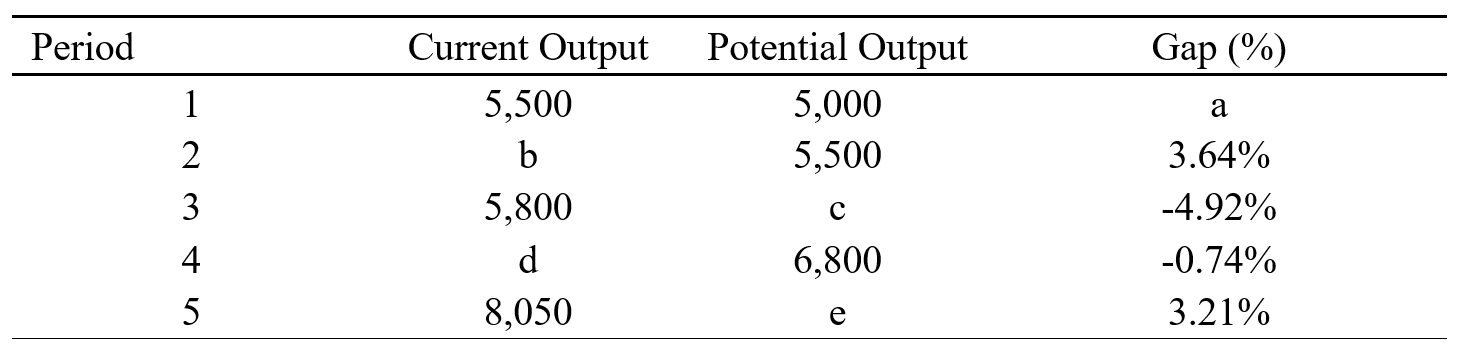
\includegraphics[width=0.8\linewidth]{figure/short-run_output}
		\end{figure}
		
		Solve a) to e). 		

		\clearpage
		
		\textbf{Solution}
		\begin{enumerate}[label=(\alph*)]
			\item $\frac{5500}{5000} - 1 = 0.1$
			\item $(1+0.0364)\times5500 = 5700 $
			\item $\frac{5800}{1-0.0492} = 6100$
			\item $(1-0.0074)\times6800 = 6749.68 $
			\item $\frac{8050}{1+0.0321} = 7800$ 
		\end{enumerate}


		\clearpage
		\item  \textbf{(20  pts)} This question centers on the IS model from Chapter 11. In a closed economy, the consumption ($C_t$), investment ($I_t$), and government purchases ($G_t$) are represented by the following equations:
		\[C_t = \bar{a}_c \bar{Y}_t\]
		\[I_t = \bar{a}_I \bar{Y}_t - \bar{b} \left(R_t - \bar{r}\right)\bar{Y}_t\]
		\[G_t = \bar{a}_G \bar{Y}_t + \bar{\beta} \widetilde{Y_t}\bar{Y}_t\]
		The equations for \( C \) and \( I \) remain the same as in the simple IS model, whereas the \( G \) equation incorporates an extension to account for automatic stabilizers -- policy that automatically adjust to economic conditions to stabilize output, such as progressive taxes and unemployment benefits.
		
		\begin{enumerate}[label=(\alph*)]
			\item \textbf{(3  pts)} Considering the extension term to account for automatic stabilizers, what is the expected range for the parameter \(\bar{\beta}\)?
			\item \textbf{(4  pts)} Derive the IS curve.
			\item \textbf{(3  pts)} How does the new extension $\bar{\beta} \widetilde{Y}$ alter the IS curve?
			\item \textbf{(4  pts)} The economy is facing a recession of $\widetilde{Y} = 0.05$. The government decided to implement a discretionary policy. By how much does the government need to increase the $\bar{a}_G$ parameter?
			\item \textbf{(2  pts)} Do automatic stabilizers support the government's discretionary policy efforts (as in part d)) to stimulate GDP?
			\item \textbf{(4  pts)} Use a graph to illustrate the effect of an increase in \(\bar{\beta}\). Draw two IS curves on a graph, with the real interest rate on the Y-axis and short-run output (\(\tilde{Y}\)) on the X-axis. Label \(IS_2\) as the IS curve with a higher absolute value of \(\bar{\beta}\) compared to \(IS_1\).
			
		\end{enumerate}
		\clearpage
		
		\textbf{Solution}
		\begin{enumerate}[label=(\alph*)]
			\item The parameter $\bar{\beta}$ would be negative to capture the idea of automatic stabilizer. As the short-run output increase (fall), the government would reduce (increase) its spending.
			\item Either of the following would be accepted
			
			\[Y_t = C_t + I_t +G_t = \bar{a}_c \bar{Y}_t+ \bar{a}_I \bar{Y}_t - \bar{b} \left(R_t - \bar{r}\right)\bar{Y}_t +\bar{a}_G \bar{Y}_t + \bar{\beta} \widetilde{Y_t} \bar{Y}_t\]
			\[\frac{Y_t}{\bar{Y}_t} = \frac{(\bar{a}_c+ \bar{a}_I+ \bar{a}_G) \bar{Y}_t - \bar{b} \left(R_t - \bar{r}\right)\bar{Y}_t  + \bar{\beta} \widetilde{Y_t} \bar{Y}_t}{\bar{Y}_t} \]
			\[\frac{Y_t}{\bar{Y}} - 1 = \tilde{Y} = (\bar{a}_c+ \bar{a}_I+ \bar{a}_G-1)  - \bar{b} \left(R_t - \bar{r}\right)  + \bar{\beta} \widetilde{Y_t}\]
			\[\widetilde{Y}_t - \bar{\beta}  \widetilde{Y_t} = \bar{a} - \bar{b} \left(R_t - \bar{r}\right)    \]
			\[\widetilde{Y_t} = \frac{1}{1-\bar{\beta}}\left[\bar{a} - \bar{b} \left(R_t - \bar{r}\right)\right]    \]
			
			\item 			
			In this setup, extension would work like a  multiplier but in a opposite effect. It is because the parameter $\bar{\beta}$ is negative. Therefore, for one percent increase in, say, $\bar{a}$ would lead to a less than one percent increase in the short-run output.
			
			\item 
			The government need to increase $\bar{a}_G$ by $5\% \times  \left(1 -  \bar{\beta}\right)$. 
			\item Given $\bar{\beta} <0$, the government would need to increase government spending by more than the fall of short-run output 
			\clearpage
			\item As the absolute value of $\beta$ increases, the slope of the IS curve would be lower. The multiplier effect becomes smaller.
			\begin{figure}[htbp!]
				\centering
				\includegraphics[width=0.7\linewidth]{"figure/IS curve"}
			\end{figure}
			
			
		\end{enumerate}

		
		\clearpage 
		\item  \textbf{(15  pts)} In a hypothetical economy, Brossard, the output gap fall to -8\% during the Great Recession in  2009. Many people believe that the multiplier was equal to 2.5. Given the equations that describe the economy:
		
		\[C_t = \bar{a}_c \bar{Y}_t + \bar{x} \widetilde{Y}_t \bar{Y}\]
		\[I_t = \bar{a}_I \bar{Y}_t - \bar{b} \left(R_t - \bar{r}\right)\bar{Y}_t\]
		\[G_t = \bar{a}_G \bar{Y}_t\]
		
		The equations for \( G \) and \( I \) remain the same as in the simple IS model, whereas the \( C \) equation incorporates an extension to account for the imperfect consumption smoothing.
		 
		\begin{enumerate}[label=(\alph*)]
			\item \textbf{(4  pts)} Derive the IS curve.
			\item \textbf{(2  pts)} What is value of $\bar{x}$? 
			\item \textbf{(2  pts)} What is value of $\bar{x}$  if the multiplier was 1.25?
			\item \textbf{(4  pts)} What would the percent change in government expenditure be to close this gap, assuming monetary policy is not being used and the multiplier is equal to 2?
			\item \textbf{(3  pts)} If there is no aggregate shock (i.e., \(\bar{a} = \bar{a}_c + \bar{a}_I + \bar{a}_G -1 = 0\)), $\bar{b} = 0.5$, $\bar{r} = 0.05$, what would the real interest rate $R_t$ be?
		\end{enumerate}
		\clearpage
		
		\textbf{Solution}
		\begin{enumerate}[label=(\alph*)]
			\item \[ C_t + I_t + G_t = Y_t = \bar{a}_c \bar{Y}_t + \bar{x} \widetilde{Y}_t \bar{Y}+ \bar{a}_I \bar{Y}_t - \bar{b} \left(R_t - \bar{r}\right)\bar{Y}_t + \bar{a}_G \bar{Y}_t\]
				\[\frac{Y_t }{\bar{Y}_t}= \bar{a}_c  + \bar{x} \widetilde{Y}_t + \bar{a}_I  - \bar{b} \left(R_t - \bar{r}\right) + \bar{a}_G  \]
				\[\frac{Y_t }{\bar{Y}_t} - 1 = \tilde{Y}_t = \left[\bar{a}_c + \bar{a}_I + \bar{a}_G - 1\right] + \bar{x} \widetilde{Y}_t   - \bar{b} \left(R_t - \bar{r}\right)   \]
				\[\tilde{Y}_t -\bar{x} \widetilde{Y}_t   = \bar{a}  - \bar{b} \left(R_t - \bar{r}\right)   \]
				\[\widetilde{Y}_t   = \frac{1}{1-\bar{x}}\left[\bar{a}  - \bar{b} \left(R_t - \bar{r}\right)\right]   \]
			\item The multiplier is $\frac{1}{1-x}$. If the multiplier is equal to 2.5,
			\[2.5 = \frac{1}{1-\bar{x}} \]
			\[\bar{x} = 0.6\]
			\item The $\bar{x} = 0.2 $
			\item The government has to increase its expenditure by $8\%/2 = 4\%$
			\item \[-0.08 = 2.5 \left[0  - 0.5 \left(R_t - 0.05\right)\right] \]
			\[-0.08 = 2.5 \left[0  - 0.5 \left(R_t - 0.05\right)\right] \]
			\[R_t = 0.114\]
			
			*Since this part of the question didn't specific the multiplier, one may use any of the three number used above.
		\end{enumerate} 

	\item  \textbf{(10 pts)}\label{P5} The quantity equation states that
	\[M_t V_t = P_t Y_t\]
	
	
	\begin{enumerate}[label=(\alph*)]
			\item \textbf{(3 pts)} 	What assumptions about $M_t$, $V_t$, and $Y_t$ are necessary for the quantity theory of money to consider the money supply as the key determinant of the price level in the long run?

			\item \textbf{(2 pts)} Show that the inflation rate is a function of \textit{only} the growth rates of money supply ($g_M$) and output ($g_Y$). State all the necessary assumptions. 

			%	
			\item \textbf{(3 pts)} Suppose the central bank announces it will gradually slow down the money supply growth. What are the likely effects on the inflation rate initially and in the long run? 

			
			\item \textbf{(2 pts)} In the long run, will the price level be higher or lower? What about the output?

	\end{enumerate}
	
	\clearpage
	\textbf{Solution}
	\begin{enumerate}[label=(\alph*)]
		\item 	
		$M_t$ is controled by the central and is exgenously given 
		
		$V_t$ is constant in the long run
		
		$Y_t$ does not affected by the money market and is determined by only the real variables, according to the classical dichotomy 
		
		Thus, $P_t$ is determined by the $M_t$ only
		
		\item 
		\[g_m + g_V = g_P + g_Y\]
		Let $g_V = 0$ as it is usually assume to be a constant. Therefore,
		\[g_P = \pi = g_m - g_Y\]
		
		\item The inflation rate would slowly decrease. In the long run, the inflation would be lower.
		
		
		\item The price level would be higher than before, even though inflation is lower, as prices would still rise but at a slower rate. Output, however, would remain unchanged, as it is determined by factors unrelated to nominal variables.
		\vspace{1cm}
		
		
	\end{enumerate}
	
	\clearpage
	\item \textbf{(35 pts)} Data Question: 
	
	\textit{You may use any program of your choice to complete the following question.}
	
	\begin{enumerate}[label=(\alph*)]
		\item \textbf{(4 pts)} Download the following data series from FRED:  
		\begin{itemize}
			\item ``Real Gross Domestic Product for Canada [NGDPRSAXDCCAQ]" covering the period from 1961Q1 to 2024Q2.
		\end{itemize}
		
		\item \textbf{(6 pts)} Compute the 5-quarter trailing moving average of Real GDP for Canada. Use this as the GDP trend and calculate the cyclical component (short-run output) as a percentage deviation from the trend.
		
		\item \textbf{(8 pts)} Following Hamilton's approach, estimate the regression model given by:
		\[
		y_{t+8} = 12614.50418 + 0.54737 y_{t} + 0.05201 y_{t-1} + 0.14761 y_{t-2} + 0.27181 y_{t-3} + \nu_{t+8}
		\]
		Using the estimated model, calculate the trend and cyclical component (as a percentage deviation from the trend) of Real GDP for Canada.
		
		\item \textbf{(8 pts)} Plot the two cyclical components obtained in part (b) and part (c) on a single graph with:
		\begin{itemize}
			\item \textbf{Y-axis:} Cyclical component values from part b) and part c).
			\item \textbf{X-axis:} Time (display only the year and month, excluding the day).
			\item \textbf{Titles:} Provide appropriate titles for the Y-axis, X-axis, and the overall chart.
		\end{itemize}
		
		\item \textbf{(8 pts)} Analyze the economic impact during the recent pandemic crisis. Based on the graph from part (d), which method provides a clearer picture of the economy?  (in 5-10 sentences)
		
		(This is an open-ended question. Your response will be evaluated based on how well you interpret the graph and your understanding of the Moving Average and Hamilton Filter methods.)
	\end{enumerate}

\clearpage
*R Code for Estimating the Model in Part (c)
\begin{lstlisting}[language=R]
	#Clear the Environment
	rm(list = ls())
	#Loading Package
	install.packages("neverhpfilter")
	library(neverhpfilter)
	library(xts)     # For time series handling
	
	#Loading Data
	# Replace ... with actual file path to the Data
	GDP_data <- read.csv(".../NGDPRSAXDCCAQ.csv")  
	GDP_data[[1]] <- as.Date(GDP_data[[1]])
	GDP <- xts(GDP_data[[2]], order.by = GDP_data[[1]])
	colnames(GDP) <- "GDP_Value"
	
	#Estimate Hamilton filter
	gdp_model <- yth_glm(GDP, h = 8, p = 4)
	summary(gdp_model)
\end{lstlisting}
%		\clearpage 
%		\item  \textbf{(15  pts)} As a policy advisor to the central bank with the objective of stabilizing inflation and economic activity, what would be your responses to the following three independent events? 
%		Examine the impact of each event on $\bar{a}$'s (be specific on which $\bar{a}$ is likely to change), the IS curve, short-run output $\widetilde{Y}$, and changes in the inflation rate $\Delta \pi$. Then, propose a policy adjustment in the interest rate to offset the change in inflation rate such that $\Delta \pi = 0$.
%		Also, for each event, illustrate the movement of the IS and MP curve on a graph of $R_t$ and $\widetilde{Y}$ and the Phillips curve on a graph of $\Delta \pi$ and $\widetilde{Y}$. Label all the points of interest and axes.  
%		\begin{enumerate}[label=(\alph*)]
%			\item [5] A surge in the stock markets significantly boosts people's wealth.
%			\item [5] Chilean citizens suddenly develop a preference for maple syrup. 
%			\item [5] Firms begin to grow anxious about the decline in consumer confidence.
%		\end{enumerate}
		
%		\clearpage
%		\textbf{Solution}
%		\begin{enumerate}[label=(\alph*)]
%			\item This would be a positive demand shock from the households. The $\bar{a}_C$ would rise, which shift the IS curve up. This implies the $\widetilde{Y}$ would rise. Using the PC, the $\Delta \pi$ would rise as well. you should recommend a rise in interest rates to reduce the gap and slower down inflation.
%			\item This would be a positive export shock from Chilean. The $\bar{a}_{EX}$ would rise, which shift the IS curve up. This implies the $\widetilde{Y}$ would rise. Using the PC, the $\Delta \pi$ would rise as well. you should recommend a rise in interest rates to reduce the gap and slower down inflation.
%			\item Both firm and consumer are permissive about the future. Therefore, both $\bar{a}_{I}$ and $\bar{a}_{C}$ would fall. You should recommend lowering the interest rates to boost the economy and close the gap.
%		\end{enumerate}		


%		\newpage 
%		\centering{This page intentionally left blank.}
%		\ % The empty page
%		
		\vfill
		
		 \centering{-- The End -- }
		
		
		
		%		\begin{solution}
			%			
			%		\end{solution}	
%		\clearpage 
%		
%		\item Was wäre, wenn es keine Luft gäbe?
%		\begin{parts} 
%			\item[5] Was würde mit Luftballons geschehen? 
%			\bonuspart[6] Wie könnten Fluggesellschaften damit umgehen?
%		\end{parts}
%		
%		\item [100] Wird es morgen schneien?
%		\begin{checkboxes}
%			\CorrectChoice Ja
%			\choice Nein
%			\choice Vielleicht
%		\end{checkboxes}
%		
%		\item Ein Name der folgenden Reihe passt nicht zu den anderen. Welcher?
%		\begin{oneparchoices}
%			\choice Donald
%			\choice Dagobert
%			\choice Daisy
%			\choice Micky
%			\CorrectChoice Balu
%		\end{oneparchoices}
		
	\end{enumerate}
	
%	\begin{center}
%		\combinedgradetable[h][questions]
%	\end{center}
	
\end{document}